\section{Results: four places}\label{results-four-places}

The creator chose four places from the first environment to rebuild: camp, two glass domes on Mars joined by a tunnel; campgrounds, the open site around them with a lander, a drilling rig and a mast; stairwell, a cut-away switchback stair in a residential block; and street, a rainy night street leading to a launch plaza. They are the three places that carried walkers in the first environment and the outdoor place that had read best under the old method. Figure 1 shows each concept beside its final render, and Table 1 summarises the scenes.

\begin{table}[tbp]
\centering\small
\caption{The four places. Objects checked and faults are from the final physics-readiness check of each scene, including its MuJoCo settle. Critic scores are the building agent's own judgement of its round-5 renders against the concept, out of 10; the old method's reviewing agents gave the same places 2, 4, 1 and 1. Films are 1920 by 1080 at 24 frames per second.}
\begin{tabular}{@{}lrrrlrr@{}}
\hline
Place & Objects & Faults & Concept view & Other views & Walkers & Film \\
\hline
camp & 711 & 0 & 7/10 & 6/10 insides & 2 & 29 s \\
campgrounds & 369 & 0 & 7/10 & 6/10 eye height & 3 & 34 s \\
stairwell & 61 & 0 & 4/10 & 6/10 insides & 2 & 24.5 s \\
street & 888 & 0 & 6/10 & 6/10 eye, 5/10 wide & 6 & 19 s \\
\hline
\end{tabular}
\end{table}

\textbf{Against the concepts.} By the critic's own scores, camp and campgrounds reach 7 out of 10 in the concept's view, street 6 and stairwell 4, against 2, 4, 1 and 1 for the same places under the per-picture method. The scores come from vision models on both sides, the old ones from reviewing agents and the new ones from the building agent's critic, and neither is a human rating; the comparison shows a change of scale rather than a calibrated measure. The renders in Figure 1 support it: the camp's two domes, their tunnel and their furnishing, the campgrounds' layout around the lander, the stairwell's cut-away flights and the street's lanterns, barriers and rain stand where the concepts place them. The critic's remaining notes are concrete. In camp everything is a pale beige and the lockers do not read as suit lockers, in campgrounds the sand ripples are too even and the sky is flat, the stairwell's view shows the building from outside rather than as the concept's cut-away and has no surroundings, and the street has boxy fronts with repeated windows and a garbled cafe sign. The street's late rain and its blotchy walls were traced to the renderer rather than to the scene, since the review's 16 samples denoised a lamp-lit haze into blotches, and reviews of places with haze now render at the films' 64 samples.

\textbf{Physics.} All four final scenes pass the physics-readiness check with no fault, including the MuJoCo settle of every prop: 711 objects in camp with its scattered rocks, 369 in campgrounds, 61 in the stairwell and 888 in the street. The check found real faults on the way, which were corrected at their source rather than tolerated. A laptop on a desk with a raised back fell 4.9 m through the desk because the settle had left out what held it, a walker's route through a loop collapsed to zero length when its legs were straightened as one path, rocks bedded deeper than 10 cm were read as unsupported, and the tunnel's skin had to be rounded to 96 points before it stopped reading as a polygon from inside.

\textbf{Walkers.} Thirteen walkers were routed and generated in the four places (Table 2, Figure 4). Twelve stay within 6.8 cm of their routes and keep at least 0.48 m from every upright solid. Eleven keep their planted feet within the 2 cm skate limit as Kimodo made them, and one street walker skates 2.9 cm; as played in the scene, foot skate reaches up to 2.9 cm for these twelve. The stairwell woman, who climbs the stair, is the exception on every measure. She strays 18 cm from her route, skates 3.6 cm in Kimodo's output and 4.7 cm as played, and passes within 0.31 m of a solid.

\begin{table}[tbp]
\centering\small
\caption{Walker measures per place, as ranges over its walkers: foot skate as Kimodo made the clip and as played in the scene, the hips' distance off the route, the least clearance from an upright solid, the peak residual force against its limit (2 percent of the body's weight under the place's gravity, Mars for camp and campgrounds, Earth for the others) and the share of frames within both residual limits.}
\begin{tabular}{@{}lrrrrrrr@{}}
\hline
 & & \multicolumn{2}{c}{Skate (cm)} & Off route & Clearance & Peak residual & Frames \\
Place & Walkers & Kimodo & played & (cm) & (m) & N (limit) & within \\
\hline
camp & 2 & 1.0--1.9 & 2.5--2.9 & 4.0--5.7 & 0.48 & 81--95 (5.7) & 74--87\,\% \\
campgrounds & 3 & 1.5--1.7 & 2.3--2.9 & 4.0--4.7 & 0.76 & 92--263 (5.6--5.7) & 56--82\,\% \\
stairwell, man & 1 & 1.7 & 1.6 & 4.0 & 0.73 & 597 (15.0) & 60\,\% \\
stairwell, woman & 1 & 3.6 & 4.7 & 18.0 & 0.31 & 1368 (15.0) & 39\,\% \\
street & 6 & 1.3--2.9 & 1.3--2.9 & 4.2--6.8 & 0.53 & 13--632 (14.9--15.2) & 79--98\,\% \\
\hline
\end{tabular}
\end{table}

\begin{figure}
\centering
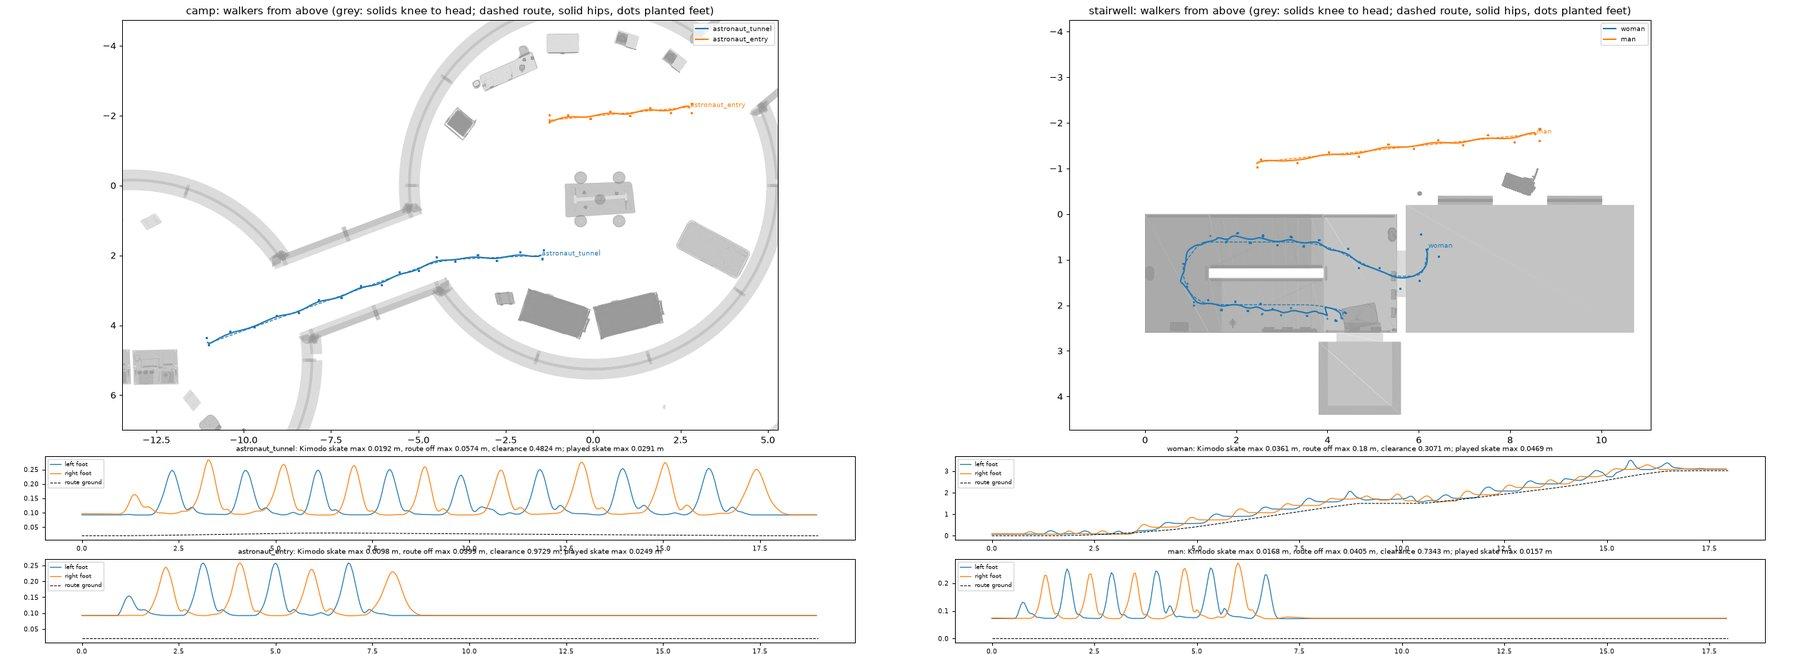
\includegraphics[width=1\linewidth,height=\textheight,keepaspectratio,alt={Walkers from above in camp (left) and the stairwell (right): grey footprints of the solids between knee and head, each walker's route dashed and its hips solid, planted feet as dots, with each walker's foot heights over time beneath. The stairwell woman's route climbs the switchback flights, and her feet follow the rising route ground.}]{figures/routes.jpg}
\caption{Walkers from above in camp (left) and the stairwell (right): grey footprints of the solids between knee and head, each walker's route dashed and its hips solid, planted feet as dots, with each walker's foot heights over time beneath. The stairwell woman's route climbs the switchback flights, and her feet follow the rising route ground.}
\end{figure}

\textbf{The residual check fails.} No walker's sim body passes the residual check over the whole clip. The best, a street walker, holds its force within the limit (13 N against 15.2 N) but not its moment (13.4 against 7.4 N m). In camp the peak residual force is 95 N against a limit of 5.7 N, while 74 to 87 percent of frames lie within both limits and the mean force is 2 to 3 N, so the failure lies in short peaks rather than throughout. The stairwell is far worse. The woman's peak reaches 1,368 N against a 15 N limit with only 39 percent of frames within, and in her film her sim body sinks about 17 cm. Section 6 discusses what this means.

\textbf{Films.} Each place's film is rendered at 1920 by 1080 and ends with its peel (Figure 5). The camp film had a final polishing round, in which its walkers walk for the whole film and the peel shows the sim body's muscles and a readable ground reaction force arrow. The other three show open faults. In campgrounds the force arrows are faint, four astronaut figures stand still and one walker starts 4.5 s late, the stairwell's man stops after 7.5 s, and in the street the peel faces the plaza's flat backdrop and most sim bodies have no centre of pressure from which to draw an arrow.

\begin{figure}
\centering
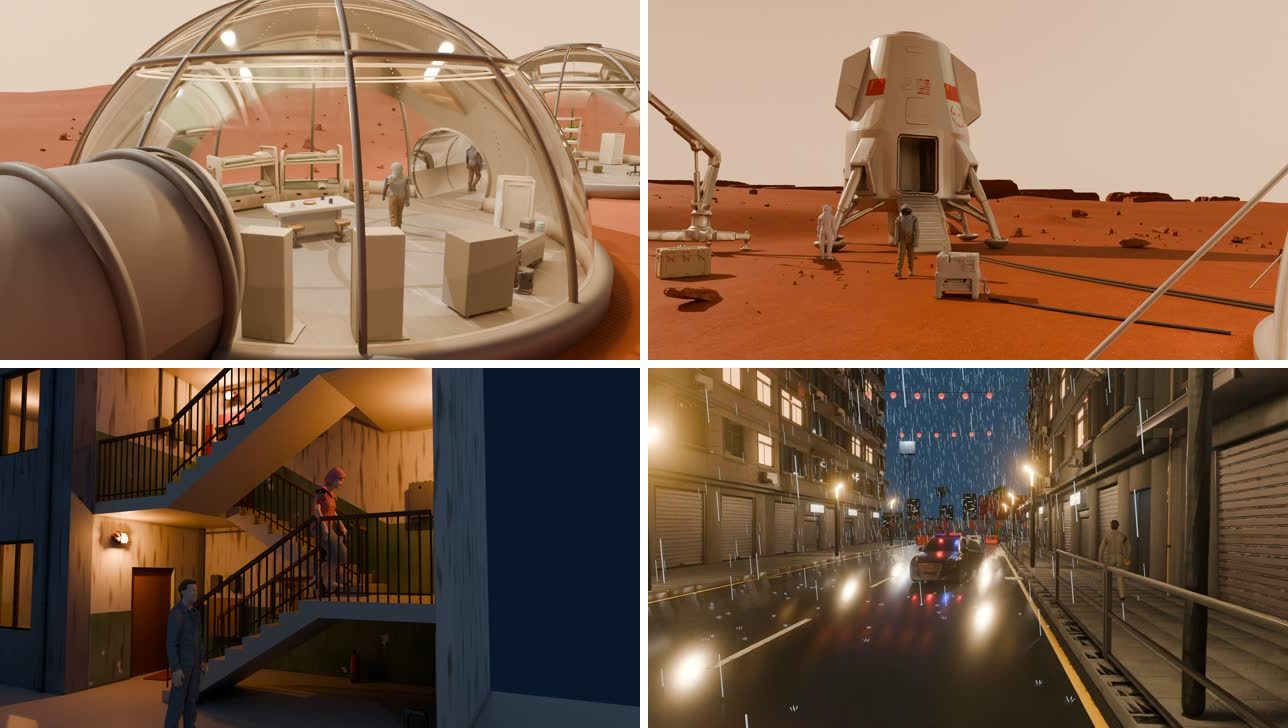
\includegraphics[width=1\linewidth,height=\textheight,keepaspectratio,alt={Frames from the four films: camp (top left), campgrounds (top right), stairwell (bottom left) and street (bottom right), each at about a third of its length.}]{figures/films.jpg}
\caption{Frames from the four films: camp (top left), campgrounds (top right), stairwell (bottom left) and street (bottom right), each at about a third of its length.}
\end{figure}

\textbf{Costs.} The four films were rendered on rented cloud graphics cards for about EUR 17. Everything else in this section was free. The building, the checks, the SAM 3 split, the TRELLIS.2 props, the walkers' Kimodo pieces and their sim bodies all ran on the creator's own computer with one 16 GB card. A TRELLIS.2 prop takes about three minutes of that card, against about EUR 0.22 (EUR 0.39 at the high estimate) for a model from the earlier paid picture-made route.
